\section{Task 2}

In this task, I placed the phone on the table without any touch or movement. 

When the phone is placed flat on a table, the accelerometer should read the gravitational acceleration on the Z-axis, while the readings on the X and Y axes should be zero.
The readings of the gyroscope should be zero in all three directions, while the magnetometer readings should reflect the magnetic field strength of the phone's current position.

Since the last moment I touched the screen to stop stream, so in calculation I throwed the last 0.1 second data away to avoid disturbances.

\subsection{True state}

\begin{figure}[H]
 \centering
 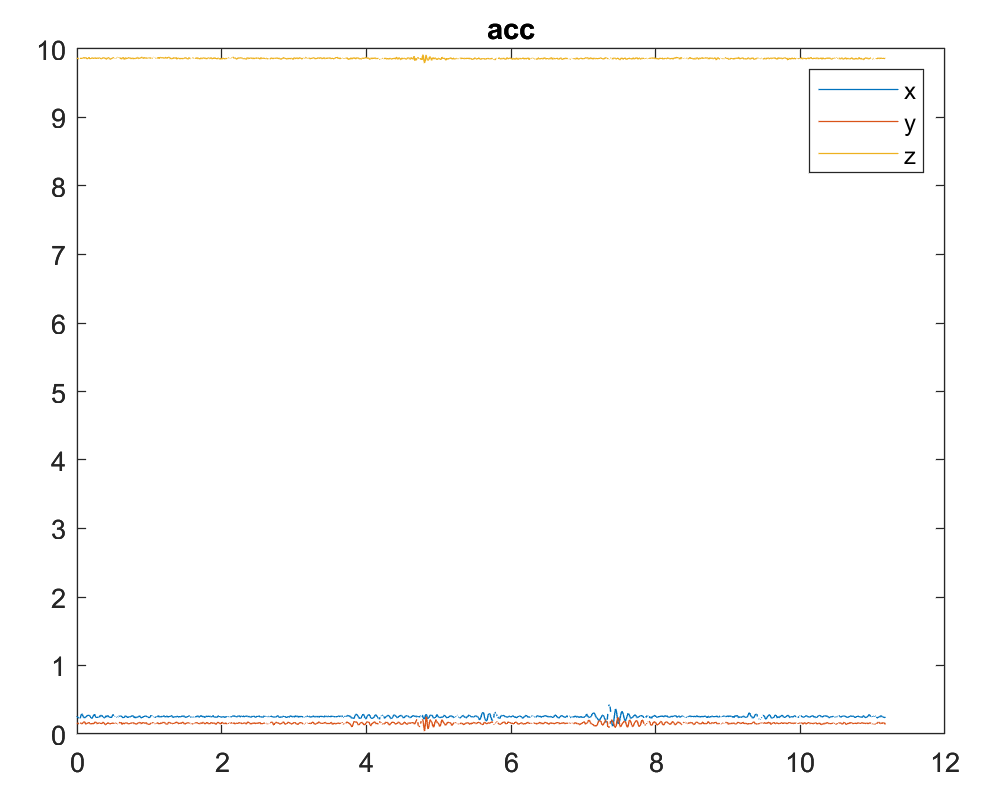
\includegraphics[width=0.7\textwidth]{images/acc.png}
 \caption{Accelerometers}
 \label{acc}
\end{figure}

\begin{figure}[H]
 \centering
 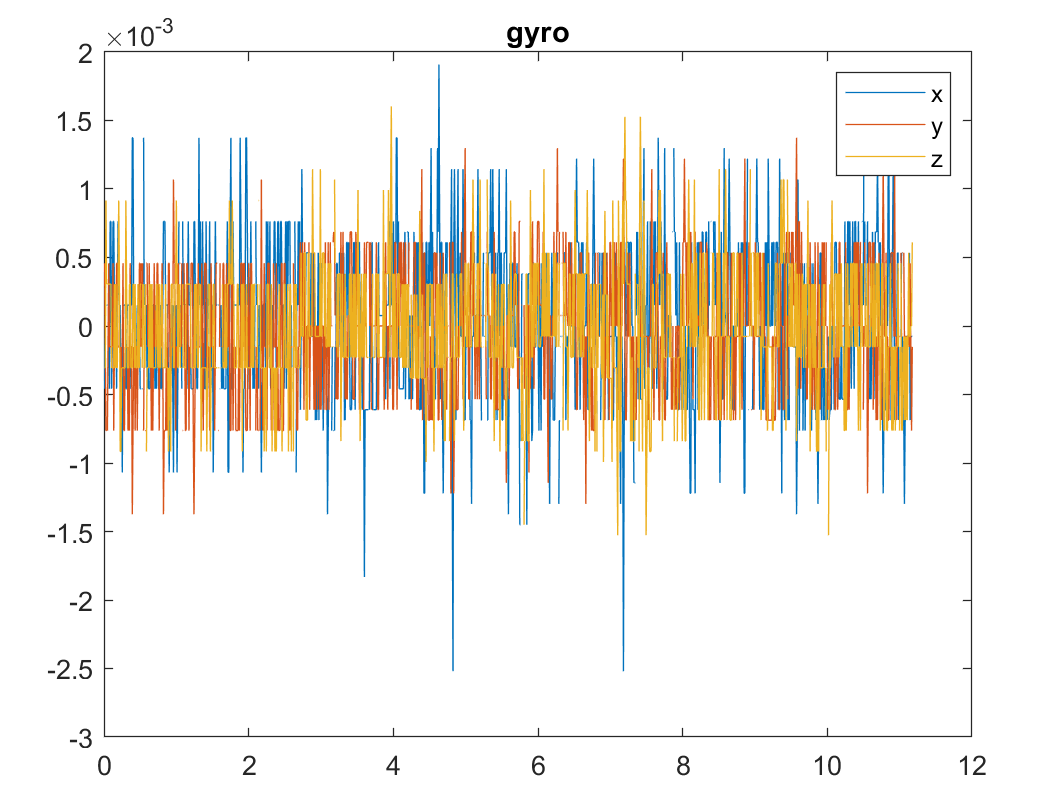
\includegraphics[width=0.7\textwidth]{images/gyroscope.png}
 \caption{Gyroscope}
 \label{gyro}
\end{figure}

\begin{figure}[H]
 \centering
 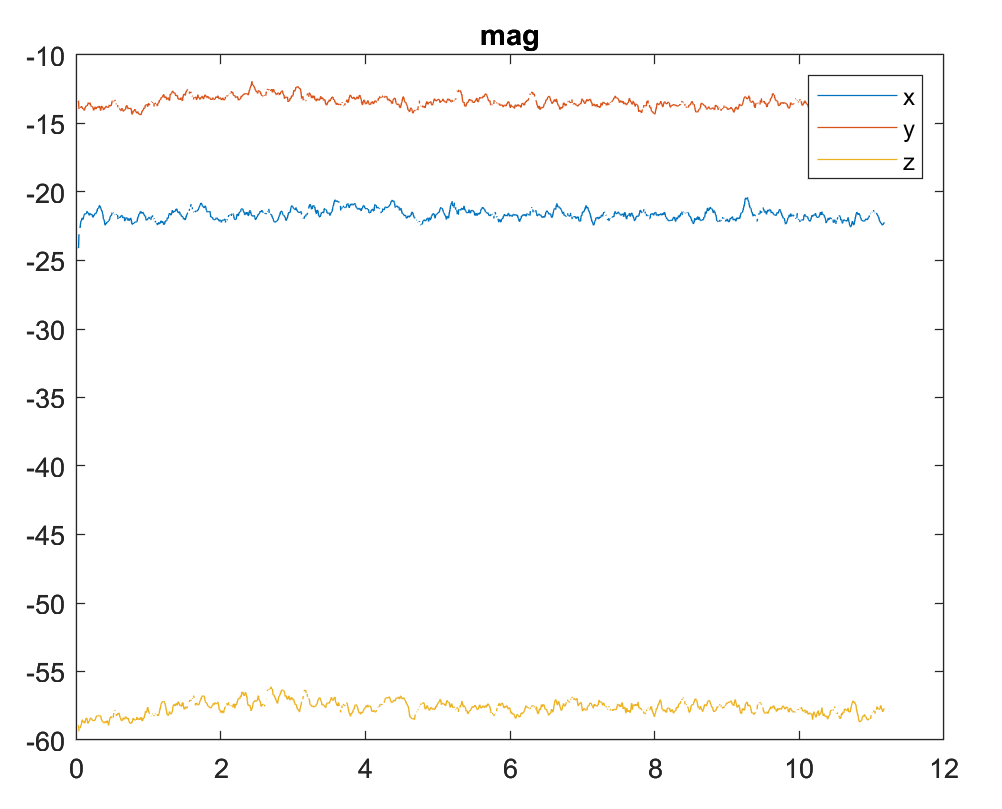
\includegraphics[width=0.7\textwidth]{images/magnetometers.png}
 \caption{Magnetometers}
 \label{mag}
\end{figure}

Through observation of the sensor plots, it is evident that when the phone is placed flat on a table, the readings from all three sensors demonstrate a consistent and stable trend without notable disturbances.


\subsection{Mean and covariance and histograms}

\begin{figure}[H]
 \centering
 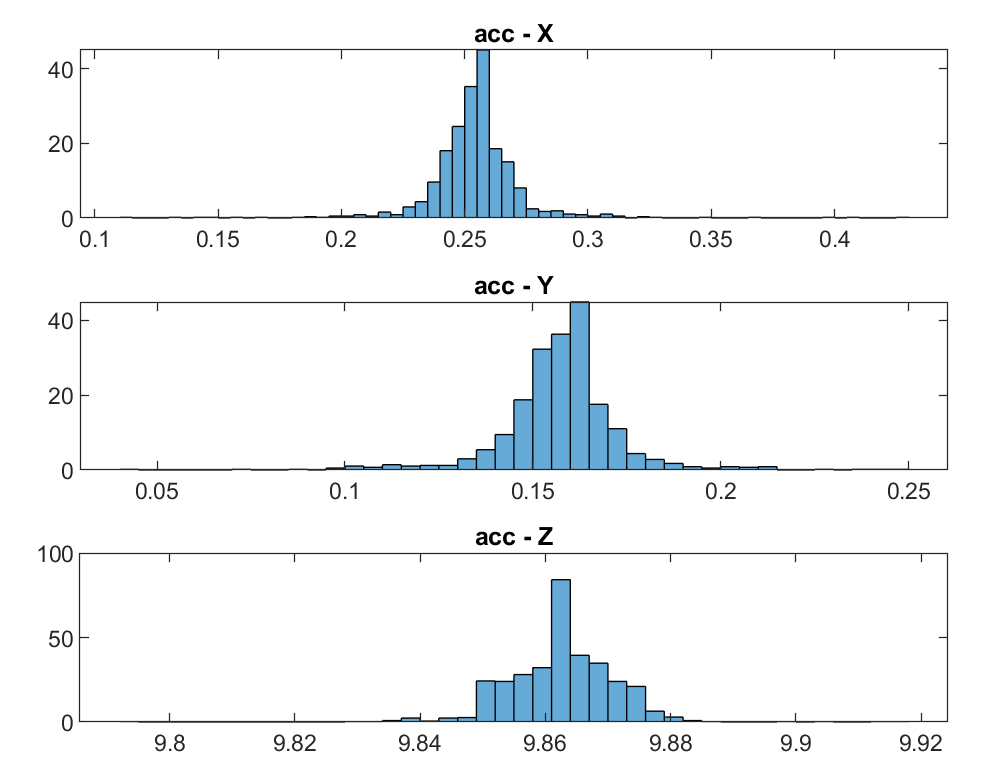
\includegraphics[width=0.7\textwidth]{images/histogramacc.png}
 \caption{Histograms for accelerometers}
 \label{hisacc}
\end{figure}

The mean of acc -X is 0.254171 , the covariance of acc -X is 0.019724  

The mean of acc -Y is 0.157052 , the covariance of acc -Y is 0.016096 

The mean of acc -Z is 9.862452 , the covariance of acc -Z is 0.008445 

\begin{figure}[H]
 \centering
 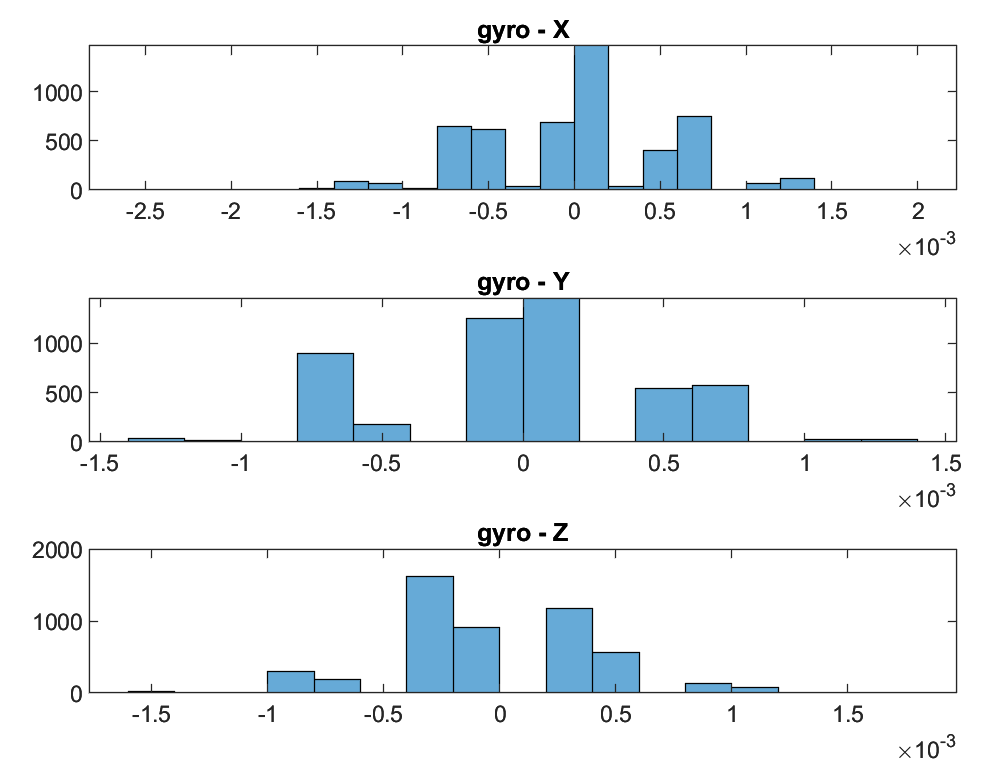
\includegraphics[width=0.7\textwidth]{images/histogramgyroscope.png}
 \caption{Histograms for gyroscope}
 \label{hisgyro}
\end{figure}


The mean of gyro -X is 0.000014 
, the covariance of gyro -X is 0.000554  

The mean of gyro -Y is -0.000031 
, the covariance of gyro -Y is 0.000449 

The mean of gyro -Z is -0.000025 
, the covariance of gyro -Z is 0.000453 

\begin{figure}[H]
 \centering
 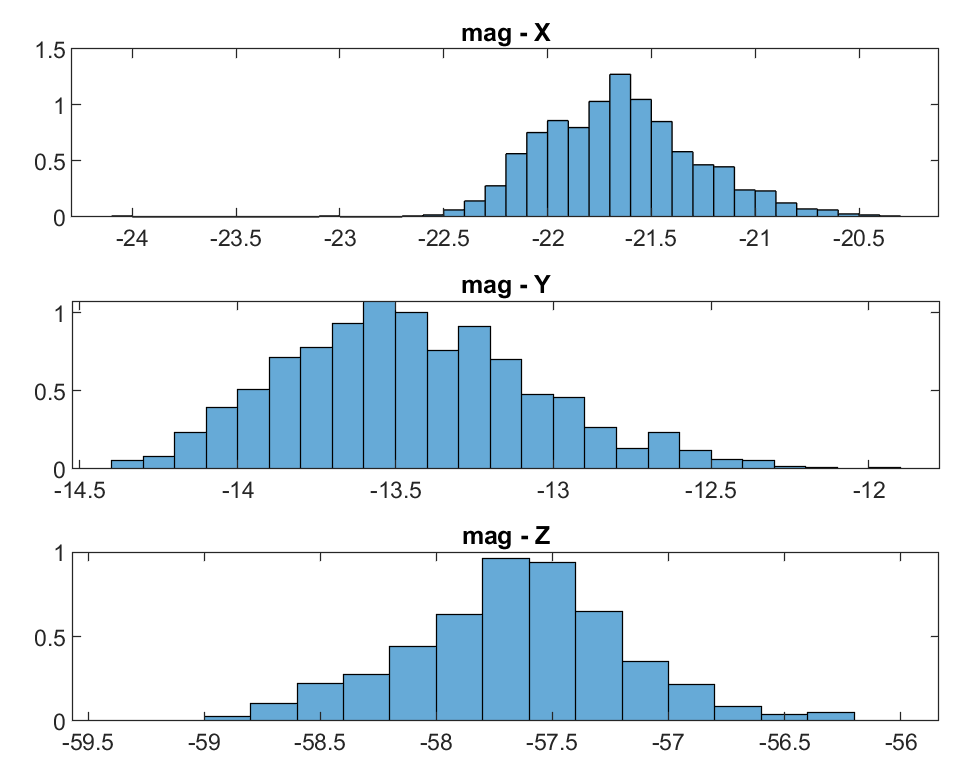
\includegraphics[width=0.7\textwidth]{images/hismagnetometer.png}
 \caption{Histograms for magnetometers}
 \label{hismag}
\end{figure}

The mean of mag -X is -21.648532 
, the covariance of mag -X is 0.377973  

The mean of mag -Y is -13.445163 
, the covariance of mag -Y is 0.401212 

The mean of mag -Z is -57.647071 
, the covariance of mag -Z is 0.477309 




The histogram of the accelerometer (acc) displays a distribution closely resembling a Gaussian shape, with a slight offset around the mean. This offset can likely be attributed to initial calibration errors during sensor measurements. Considering the protrusion of the rear camera on my phone, it is plausible that the mean offset of the accelerometer is influenced by the components of gravitational acceleration along the corresponding coordinate axes. As the phone is unlikely to be placed on a table for future measurements, this error can be mitigated. Therefore, it is reasonable to treat the accelerometer noise as Gaussian noise.

The histogram of the gyroscope (gyro) does not precisely align with a Gaussian distribution. This discrepancy may be due to the extremely small measurement errors of the gyroscope. Even if there are some offsets, the histogram shape may not exhibit a pronounced Gaussian distribution due to the minimal presence of noise. The noise in the gyroscope is exceptionally small, rendering it highly reliable. Therefore, during the subsequent tuning process, it can be assumed to have negligible measurement model noise and set to zero.

The histogram of the magnetometer (mag) exhibits a shape resembling a Gaussian distribution, albeit with an overall offset. This offset could be influenced by environmental noise in the magnetic field or biases in the magnetometer. To ensure accurate measurements, it is recommended to calibrate the magnetometer based on the current environment before each use, taking into account the specific requirements of the subsequent content.


In the subsequent experiments, I placed the mobile phone on a roll of paper to ensure that the mobile phone's XY plane was parallel to the table as much as possible. This also extended the measurement time. Therefore, new measurement values were used in the last few tasks, but they were all based on the \texttt{calculation} function.

